
当然,专业项目的最后一个要素是文档。其分为两类:

\begin{itemize}
\item 
技术文档(接口、设计、类和文件)

\item 
一般文档(所有其他非技术文档)
\end{itemize}

正如在第10章中看到的,使用Doxygen可以使用CMake自动生成很多技术文档。

\subsubsubsection{12.7.1\hspace{0.2cm}自动生成文档}

需要提到的一点是:有些项目在构建阶段生成文档,并将其与项目的其余部分打包,这是个人喜好的问题。对于这个项目,不会这样做。您可能有很好的理由选择其他方式(例如在线托管文档)。

图12.7展示了这个过程中使用的执行流的概述:

\begin{center}
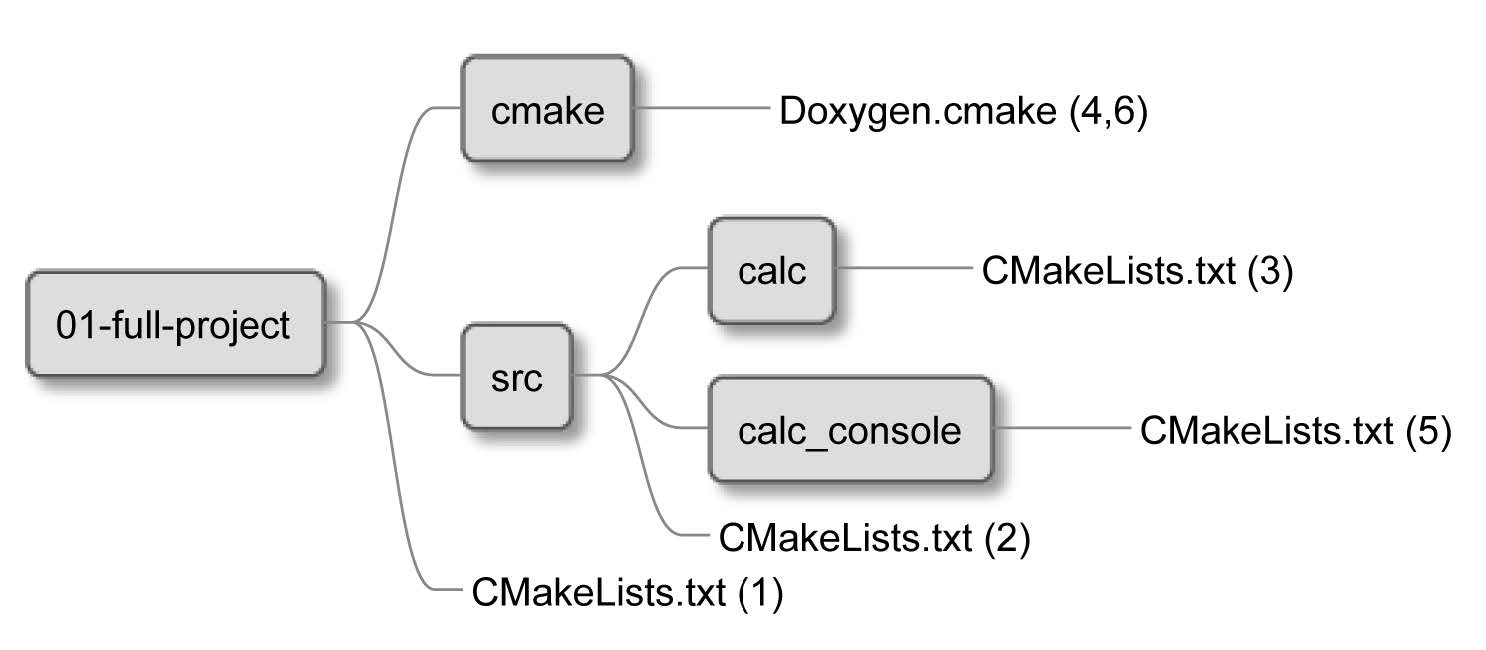
\includegraphics[width=0.6\textwidth]{content/3/chapter12/images/7.jpg}\\
图12.7 用于生成文档的文件
\end{center}

我们的生成文档目标,将创建另一个CMake实用程序模块Doxygen。这里可以使用Doxygen查找模块,并下载Doxygen的-awesome-css主题:

\begin{lstlisting}[style=styleCMake]
# chapter-12/01-full-project/cmake/Doxygen.cmake (fragment)

find_package(Doxygen REQUIRED)
include(FetchContent)
FetchContent_Declare(doxygen-awesome-css
	GIT_REPOSITORY
		https://github.com/jothepro/doxygen-awesome-css.git
	GIT_TAG
		v1.6.0
)
FetchContent_MakeAvailable(doxygen-awesome-css)
\end{lstlisting}

然后,需要一个函数来创建生成文档的目标。这将借鉴第10章介绍的代码,并对其进行修改以支持多个目标。

\begin{lstlisting}[style=styleCMake]
# chapter-12/01-full-project/cmake/Doxygen.cmake (continued)

function(Doxygen target input)
	set(NAME "doxygen-${target}")
	set(DOXYGEN_HTML_OUTPUT
		${PROJECT_BINARY_DIR}/${NAME})
	set(DOXYGEN_GENERATE_HTML YES)
	set(DOXYGEN_GENERATE_TREEVIEW YES)
	set(DOXYGEN_HAVE_DOT YES)
	set(DOXYGEN_DOT_IMAGE_FORMAT svg)
	set(DOXYGEN_DOT_TRANSPARENT YES)
	set(DOXYGEN_HTML_EXTRA_STYLESHEET
		${doxygen-awesome-css_SOURCE_DIR}/doxygenawesome.css)
	doxygen_add_docs(${NAME}
		${PROJECT_SOURCE_DIR}/${input}
			COMMENT "Generate HTML documentation"
	)
endfunction()
\end{lstlisting}

现在,需要通过为库目标调用来使用这个函数:

\begin{lstlisting}[style=styleCMake]
# chapter-12/01-full-project/src/calc/CMakeLists.txt (continued)

# ... calc_static target definition
# ... testing and program analysis modules
include(Doxygen)
Doxygen(calc src/calc)
\end{lstlisting}

我们为控制台可执行文件调用它:

\begin{lstlisting}[style=styleCMake]
# chapter-12/01-full-project/src/calc_console/CMakeLists.txt (continued)

# ... calc_static target definition
# ... testing and program analysis modules
include(Doxygen)
Doxygen(calc_console src/calc_console)

add_executable(calc_console bootstrap.cpp)
target_link_libraries(calc_console calc_console_static)
\end{lstlisting}

项目中添加了两个新目标: doxygen-calc和dooxygen-calc\_console,并且可以按需生成技术文档。

还需要提供其他文件么?

\subsubsubsection{12.7.2\hspace{0.2cm}非技术性文件}

专业的项目应该始终包含至少两个存储在顶层目录中的文档:

\begin{itemize}
\item 
README – 项目概述

\item 
LICENSE – 指定项目的软件许可证
\end{itemize}

也可以考虑添加以下内容:

\begin{itemize}
\item 
INSTALL – 描述安装所需的步骤

\item 
CHANGELOG – 列出在不同版本中发生的重要更改

\item 
AUTHORS – 若项目有多个贡献者,则包含名单和联系方式

\item 
BUGS – 告知已知的错误,并指导如何报告新错误
\end{itemize}

当涉及到这些文件时,CMake本身并没有发挥声明作用——没有自动的行为或脚本可以使用这些文件是C++项目的重要组成部分,为了完整性应该将其涵盖。作为参考,这里将提供一个最小的示例文件集,从一个简短的README文件开始:

\begin{lstlisting}[style=stylePython]
# chapter-12/01-full-project/README.md

# Calc Console
Calc Console is a calculator that adds two numbers in a
terminal. It does all the math by using a **Calc** library.
This library is also available in this package.

This application is written in C++ and built with CMake.

## More information
- Installation instructions are in the INSTALL file
- License is in the LICENSE file
\end{lstlisting}

这句话很短,可能有点傻。注意扩展名.md——代表Markdown,这是一种基于文本的格式化语言,易于阅读。像GitHub这样的网站和许多文本编辑器将以丰富的格式呈现这些文件。

INSTALL文件看起来像这样:

\begin{lstlisting}[style=stylePython]
# chapter-12/01-full-project/INSTALL

To install this software you'll need to provide the following:

- C++ compiler supporting C++17
- CMake >= 3.20
- GIT
- Doxygen + Graphviz
- CPPCheck
- Valgrind

This project also depends on GTest, GMock and FXTUI. This
software is automatically pulled from external repositories
during the installation.

To configure the project type:
cmake -B <temporary-directory>

Then you can build the project:
cmake --build <temporary-directory>

And finally install it:
cmake --install <temporary-directory>

To generate the documentation run:
cmake --build <temporary-directory> -t doxygen-calc
cmake --build <temporary-directory> -t doxygen-calc_console
\end{lstlisting}

这个文件有点长,但涵盖了最重要的需求、步骤和命令,可以很好地满足需求。

LICENSE文件有点棘手,因为需要版权法方面的一些专业知识(或其他)。我们不需要自己编写所有的条款,而是可以像许多其他项目一样使用现成的软件许可。对于这个项目,将使用MIT许可。根据具体项目的需要,可能想要选择其他的东西——查看扩展阅读部分,以获得一些有用的参考:

\begin{lstlisting}[style=stylePython]
# chapter-12/01-full-project/LICENSE

Copyright 2022 Rafal Swidzinski

Permission is hereby granted, free of charge, to any person
obtaining a copy of this software and associated documentation
files (the "Software"), to deal in the Software without
restriction, including without limitation the rights to use,
copy, modify, merge, publish, distribute, sublicense, and/
or sell copies of the Software, and to permit persons to whom
the Software is furnished to do so, subject to the following
conditions:

The above copyright notice and this permission notice shall be
included in all copies or substantial portions of the Software.

THE SOFTWARE IS PROVIDED "AS IS", WITHOUT WARRANTY OF ANY
KIND, EXPRESS OR IMPLIED, INCLUDING BUT NOT LIMITED TO THE
WARRANTIES OF MERCHANTABILITY, FITNESS FOR A PARTICULAR PURPOSE
AND NONINFRINGEMENT. IN NO EVENT SHALL THE AUTHORS OR COPYRIGHT
HOLDERS BE LIABLE FOR ANY CLAIM, DAMAGES OR OTHER LIABILITY,
WHETHER IN AN ACTION OF CONTRACT, TORT OR OTHERWISE, ARISING
FROM, OUT OF OR IN CONNECTION WITH THE SOFTWARE OR THE USE OR
OTHER DEALINGS IN THE SOFTWARE.
\end{lstlisting}

最后是CHANGELOG,最好跟踪文件中的更改,以便使用项目的开发人员可以轻松地找到支持所需特性的版本。例如,在0.8.2版本中向库添加了乘法特性,这样说可能会很有用。像下面这样简单的方法已经很有帮助了:

\begin{lstlisting}[style=stylePython]
# chapter-12/01-full-project/CHANGELOG

1.0.0 Public version with installer
0.8.2 Multiplication added to the Calc Library
0.5.1 Introducing the Calc Console application
0.2.0 Basic Calc library with Sum function
\end{lstlisting}

我们的项目现在已经完成了——可以构建、测试、生成包,将所有源代码上传到存储库,并发布工件。当然,若这可以自动发生,也可以使用CI/CD流水,这就更容易了。但那是另一本书所要做的事情了。












